\section{前沿的评价}
\label{sec:moo-front-evaluation}

算法交出了一组候选，这组候选好不好？真实前沿通常是未知的，所以要明确：在固定目标尺度和计算预算的情况下，能报告哪些可计算的量，它们分别说明什么。本节先看单个候选的质量，再看整组候选的覆盖范围。

\subsection{候选质量}
\label{sec:moo-candidate-quality}

一个候选点要检查什么？这一小节列出三项检查：是否可行，它自己的子问题解得好不好，以及是否还有共同下降的余地。

\paragraph{约束违反}
第一项是可行性。对每个候选报告最大约束违反量
\begin{equation}
 \mathrm{viol}(\bm{x})=\max\Bigl\{\max_j\,[g_j(\bm{x})]_+,\ \max_k\,\lvert h_k(\bm{x})\rvert\Bigr\},
 \label{eq:moo-violation}
\end{equation}
其中$[v]_+=\max\{v,0\}$。违反约束的点不能参与支配比较：稍微违反约束的点常常看起来更好，让它留在候选集中，会把真正可行的点错误地淘汰掉。

\paragraph{两种残差}
第二项是该候选作为优化结果的误差，这要看它是怎么得来的，要回答的问题也不同。

若候选来自权重$\bm{w}$的无约束加权和，就看它作为这个单目标问题的解有多准，用\term{标量子问题误差}（scalar subproblem error）衡量，光滑无约束时常用梯度范数
\begin{equation}
 \rho_{\bm{w}}(\bm{x})=\Bigl\lVert\sum_{i=1}^mw_i\nabla f_i(\bm{x})\Bigr\rVert_2.
 \label{eq:moo-scalar-residual}
\end{equation}

若候选是作为Pareto驻定点提交的，要看的是\term{共同下降残差}（common descent residual）$\lVert\bar{\bm{g}}(\bm{x})\rVert_2$，也就是式~\eqref{eq:moo-min-norm}中的最短长度。

这两种残差回答的问题不同。由于$\bar{\bm{g}}$是所有凸组合中最短的，对任意$\bm{w}\in\Delta_m$，
\begin{equation}
 \lVert\bar{\bm{g}}(\bm{x})\rVert_2\leq\rho_{\bm{w}}(\bm{x}).
 \label{eq:moo-residual-order}
\end{equation}
标量残差小，共同下降残差必定也小；反过来不成立。

在例~\eqref{eq:moo-iso}上算两个候选，权重都取$(1/2,1/2)$。第一个候选$\hat{\bm{x}}=(0.9,0.1)$在解集上，
\[
 \bm{g}_1=(-0.1,0.1),\qquad\bm{g}_2=(0.9,-0.9).
\]
两个梯度反向，$\lVert\bar{\bm{g}}\rVert_2=0$，它是驻定的。但
\[
 \rho_{\bm{w}}=\lVert(0.4,-0.4)\rVert_2\approx0.566.
\]
所以这个点是前沿上的一点，却不是“两项同样重要”这个偏好下的解。

第二个候选$\hat{\bm{x}}=(0.6,0.5)$略微偏离解集，
\[
 \bm{g}_1=(-0.4,0.5),\qquad\bm{g}_2=(0.6,-0.5).
\]
由式~\eqref{eq:moo-theta-two}算出$\theta^\star=0.55$，$\bar{\bm{g}}=(0.05,0.05)$，其长度约为$0.071$；而$\rho_{\bm{w}}=\lVert(0.1,0)\rVert_2=0.1$。两个残差都不为零，式~\eqref{eq:moo-residual-order}成立。

图~\ref{fig:moo-candidate-residual}把这种差别沿着整条线段画了出来：解集上共同下降残差处处为零，标量残差却只在$s=1/2$处为零。偏离解集的距离加入后，两种残差都不再为零。所以报告残差时要说清楚是哪一种。若目的是“实现这个偏好”，就看$\rho_{\bm{w}}$；若目的是“候选不能再被一阶共同改进”，就看$\lVert\bar{\bm{g}}\rVert_2$。

\begin{BookInlineFigure}
  \centering
  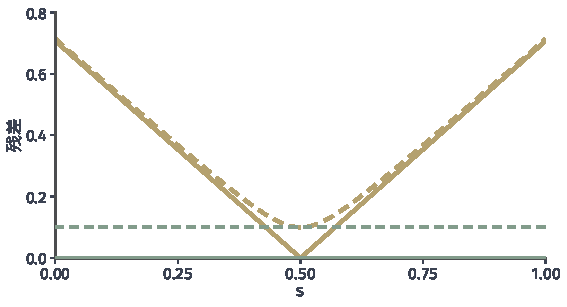
\includegraphics[width=96mm]{figures/05-optimization/07-multiple-criteria-and-nested-optimization/matplotlib/moo-candidate-residual/figure.pdf}
  \caption{例~\eqref{eq:moo-iso}中两种残差沿$\bm{x}(s)=(1-s,s)+\delta(1,1)/\sqrt2$的变化。绿线是共同下降残差，黄线是$\bm{w}=(1/2,1/2)$的标量残差，实线为$\delta=0$，虚线为$\delta=0.1$。}
  \label{fig:moo-candidate-residual}
\end{BookInlineFigure}

约束问题中，$\rho_{\bm{w}}$和$\lVert\bar{\bm{g}}\rVert_2$要换成相应的KKT残差，即式~\eqref{eq:moo-kkt}的左端在给定乘子下的范数，再加上互补松弛的误差。

\paragraph{筛选的局限}
第三项是把候选集中被支配的点剔除，用第~\ref{sec:moo-scan}节的存档方法即可。剔除之后剩下的点互不支配，但这只是在已有候选之间比较。

图~\ref{fig:moo-hidden-dominator}中，$A,B,C,D$互不支配。如果有一个没被算到的方案$\bm{P}=(3,3)$，它支配$C$，粉色区域中的方案都比它差。有限候选之间的筛选，永远不能证明不存在尚未找到的支配方案。

\begin{BookInlineFigure}
  \centering
  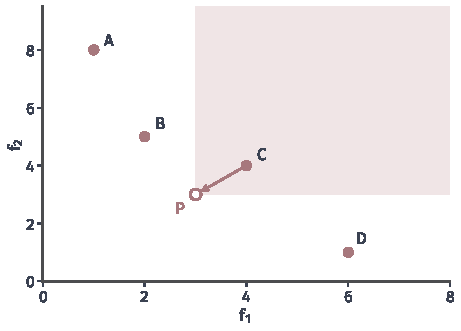
\includegraphics[width=78mm]{figures/05-optimization/07-multiple-criteria-and-nested-optimization/matplotlib/moo-hidden-dominator/figure.pdf}
  \caption{有限候选的筛选不足以判定最优。红点$A,B,C,D$互不支配，尚未找到的方案$\bm{P}=(3,3)$（红色空心点）却支配$C$，$C$落在$\bm{P}$的被支配区域（粉色）中。}
  \label{fig:moo-hidden-dominator}
\end{BookInlineFigure}

证明一个候选是全局Pareto最优的办法有两种：问题是凸的，用定理~\ref{thm:moo-kkt-sufficient}；或者全局求解一个能够选中它的标量子问题。两种都不能依靠候选之间的比较。

\subsection{覆盖范围}
\label{sec:moo-coverage}

单个候选合格，整组未必合格，它们可能都挤在前沿的一小段上。这一小节讨论怎样用数字描述整组候选的质量，以及每个数字的局限。

\paragraph{超体积}
取一个比所有候选都差的\term{参考点}$\bm{r}$，也就是各分量都大于候选相应分量的点。候选集$\bm{S}$支配的、并被$\bm{r}$界住的区域的体积称为\term{超体积}（hypervolume）：
\begin{equation}
 \mathrm{HV}(\bm{S};\bm{r})=\mathrm{vol}\Bigl(\bigcup_{\bm{y}\in\bm{S}}\{\bm{z}:\bm{y}\leq\bm{z}\leq\bm{r}\}\Bigr).
 \label{eq:moo-hv}
\end{equation}
一个指标把“离前沿多近”和“覆盖多宽”都包含进来：候选越靠前沿，被支配区域越大；候选越分散，并集越大。

两个目标时超体积可以按条带求和。把候选按$f_1$从小到大排序，设互不支配，记第$i$点为$(y_{1,i},y_{2,i})$，$i=1,\ldots,N$，并约定$y_{1,N+1}=r_1$。则
\begin{equation}
 \mathrm{HV}=\sum_{i=1}^{N}(y_{1,i+1}-y_{1,i})(r_2-y_{2,i}).
 \label{eq:moo-hv-2d}
\end{equation}

对$A,B,C,D$取$\bm{r}=(8,9)$，四个条带的面积是
\[
 (2-1)(9-8)=1,\quad(4-2)(9-5)=8,\quad(6-4)(9-4)=10,\quad(8-6)(9-1)=16,
\]
总和$\mathrm{HV}=35$，见图~\ref{fig:moo-hypervolume}。把$E$或$F$加进来，超体积不变，因为它们支配的区域已经被覆盖。把$C$去掉，超体积变成$33$，$C$独占的贡献是$(6-4)(5-4)=2$。

\begin{BookInlineFigure}
  \centering
  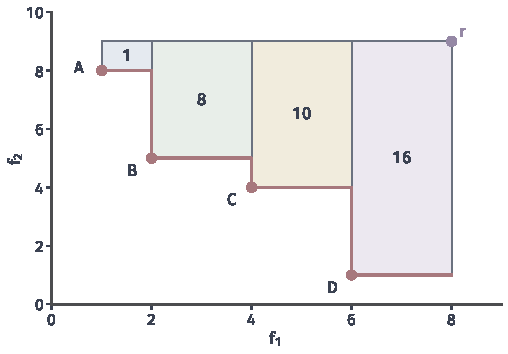
\includegraphics[width=86mm]{figures/05-optimization/07-multiple-criteria-and-nested-optimization/matplotlib/moo-hypervolume/figure.pdf}
  \caption{$A,B,C,D$的超体积，参考点$\bm{r}=(8,9)$。彩色条带的面积分别是$1,8,10,16$，合计$35$。红色阶梯线是这组候选支配区域的左下边界。}
  \label{fig:moo-hypervolume}
\end{BookInlineFigure}

超体积的好处在于它和支配关系是相容的。

\begin{theorem}[超体积的单调性]
\label{thm:moo-hv-monotone}
设$\bm{S},\bm{S}'$的所有点都逐分量不大于$\bm{r}$。若对每个$\bm{y}'\in\bm{S}'$，存在$\bm{y}\in\bm{S}$使$\bm{y}\leq\bm{y}'$，则
\begin{equation}
 \mathrm{HV}(\bm{S};\bm{r})\geq\mathrm{HV}(\bm{S}';\bm{r}).
 \label{eq:moo-hv-monotone}
\end{equation}
\end{theorem}

\begin{proof}
若$\bm{y}\leq\bm{y}'\leq\bm{z}\leq\bm{r}$，则$\bm{y}\leq\bm{z}\leq\bm{r}$。所以$\bm{S}'$对应的并集包含在$\bm{S}$对应的并集中，体积不减。
\end{proof}

也就是说，把一组候选换成支配它们的另一组，超体积不会下降。

\paragraph{参考点和尺度}
超体积不是一个自足的数字，它依赖参考点。设$\bm{S}_1=\{(1,6),(6,1)\}$，$\bm{S}_2=\{(3,3)\}$。取$\bm{r}=(7,7)$，由式~\eqref{eq:moo-hv-2d}，
\[
 \mathrm{HV}(\bm{S}_1)=5\times1+1\times6=11,\qquad\mathrm{HV}(\bm{S}_2)=4\times4=16.
\]
$\bm{S}_2$更好。取$\bm{r}=(20,20)$，
\[
 \mathrm{HV}(\bm{S}_1)=5\times14+14\times19=336,\qquad\mathrm{HV}(\bm{S}_2)=17\times17=289.
\]
$\bm{S}_1$更好。参考点越远，越看重前沿的两端，见图~\ref{fig:moo-hv-reference}。比较不同算法时，参考点必须事先固定，并且和结果一起报告。

\begin{BookInlineFigure}
  \centering
  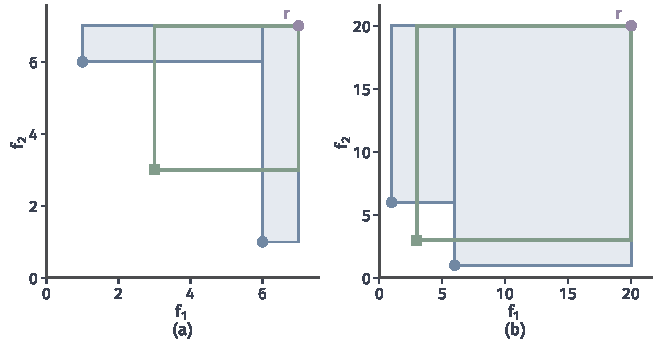
\includegraphics[width=112mm]{figures/05-optimization/07-multiple-criteria-and-nested-optimization/matplotlib/moo-hv-reference/figure.pdf}
  \caption{超体积比较依赖参考点。蓝色区域属于$\bm{S}_1=\{(1,6),(6,1)\}$，绿色方框属于$\bm{S}_2=\{(3,3)\}$。(a)$\bm{r}=(7,7)$，$\bm{S}_2$较大。(b)$\bm{r}=(20,20)$，$\bm{S}_1$较大。}
  \label{fig:moo-hv-reference}
\end{BookInlineFigure}

尺度的影响也要说明。把目标$k$乘以$c>0$，参考点相应乘以$c$，所有超体积同乘$c$，比较结果不变。但把目标归一化时，若参考范围随候选集而变，每组候选用的就是不同的尺子，比较便失去了共同的基准。

\paragraph{空缺与取舍范围}
超体积把很多信息压成一个数，可能掩盖分布上的差别。还要报告相邻候选之间的最大间距和目标的取舍范围。

在例~\eqref{eq:moo-iso}的前沿上，用$s$值表示候选，取$\bm{S}_1:\ s=0.1,0.5,0.9$与$\bm{S}_2:\ s=0.24,0.515,0.975$。取$\bm{r}=(1.2,1.2)$，两者的超体积都等于$1.0897$，见图~\ref{fig:moo-coverage-distance}。可是把前沿两端也算上，$\bm{S}_1$的最大相邻间距约为$0.609$，$\bm{S}_2$约为$0.724$，$\bm{S}_2$在靠$f_2$轴的一端空出了更大的一段。

\begin{BookInlineFigure}
  \centering
  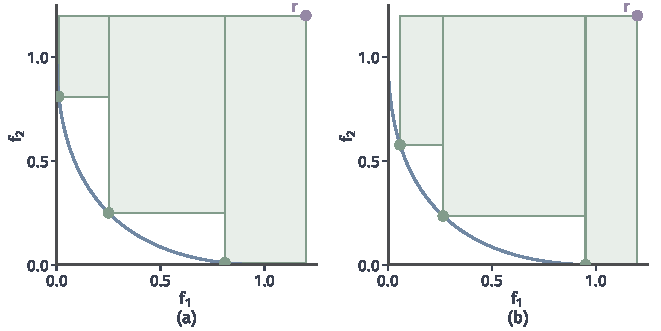
\includegraphics[width=112mm]{figures/05-optimization/07-multiple-criteria-and-nested-optimization/matplotlib/moo-coverage-distance/figure.pdf}
  \caption{两组超体积相同（$\bm{r}=(1.2,1.2)$，$\mathrm{HV}=1.0897$）的候选，蓝线是真实前沿。(a)$s=0.1,0.5,0.9$。(b)$s=0.24,0.515,0.975$，最大相邻间距更大。}
  \label{fig:moo-coverage-distance}
\end{BookInlineFigure}

\paragraph{到参考前沿的距离}
若有可信的参考前沿$\bm{R}$，比如问题有解析解，或者是长时间计算汇总的结果，可以进一步计算候选集与它的距离。两个常用的量是\term{世代距离}（generational distance，GD）和\term{反向世代距离}（inverted generational distance，IGD）：
\begin{equation}
 \begin{aligned}
  \mathrm{GD}&=\frac{1}{\lvert\bm{S}\rvert}\sum_{\bm{y}\in\bm{S}}\min_{\bm{p}\in\bm{R}}\lVert\bm{y}-\bm{p}\rVert_2,\\
  \mathrm{IGD}&=\frac{1}{\lvert\bm{R}\rvert}\sum_{\bm{p}\in\bm{R}}\min_{\bm{y}\in\bm{S}}\lVert\bm{y}-\bm{p}\rVert_2.
 \end{aligned}
 \label{eq:moo-gd-igd}
\end{equation}

GD看候选离前沿有多近，IGD看前沿被候选覆盖得多好。图~\ref{fig:moo-coverage-distance}的两组候选都在前沿上，GD都是零。IGD用$1001$个参考点计算，$\bm{S}_1$约为$0.143$，$\bm{S}_2$约为$0.163$，这里区分出了两组候选的覆盖差别。

这些量都要有参考前沿才能算。若参考前沿是其他算法的结果，算出的就只是相对的差别，不是真实误差。

\paragraph{多个指标一起看}
图~\ref{fig:moo-nsga-indicators}是图~\ref{fig:moo-nsga-run}那次运行的指标曲线，参考点取$\bm{r}=(1.1,1.1)$。超体积在第$40$代已经到$0.512$，真实前沿对应的值是$0.5433$，第$200$代是$0.5245$。到参考前沿的平均距离第$100$代约为$0.0141$，第$200$代约为$0.0153$，并不单调。

\begin{BookInlineFigure}
  \centering
  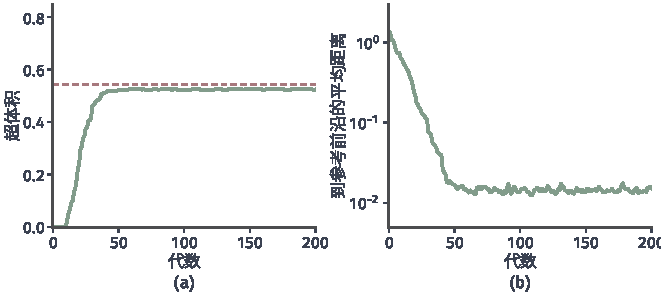
\includegraphics[width=112mm]{figures/05-optimization/07-multiple-criteria-and-nested-optimization/matplotlib/moo-nsga-indicators/figure.pdf}
  \caption{NSGA-II运行中的指标，问题为式~\eqref{eq:moo-zdt}。(a)超体积，$\bm{r}=(1.1,1.1)$，红色虚线是真实前沿的值$0.5433$。(b)种群第一层到参考前沿的IGD，纵轴为对数。曲线后段不是单调的。}
  \label{fig:moo-nsga-indicators}
\end{BookInlineFigure}

种群只有$40$个点，覆盖不了整条曲线，超体积不会达到$0.5433$，这个差额来自有限的点数。同一种群的第一层不断变化时，IGD也可以上下波动。不能用一个集合指标代替所有判断。表~\ref{tab:moo-indicators}列出各个量各自回答的问题。

\begin{BookInlineTable}
  \centering
  \caption{候选集的常用评价量。}
  \label{tab:moo-indicators}
  \begin{tabular}{@{}lll@{}}
    \toprule
    量 & 回答的问题 & 需要的条件\\
    \midrule
    约束违反 & 是否可行 & 约束函数\\
    标量残差 & 这次偏好解得准不准 & 权重或阈值\\
    共同下降残差 & 还能否一阶共同改进 & 梯度\\
    超体积 & 支配区域多大 & 固定的$\bm{r}$与尺度\\
    最大间距 & 前沿上有无大空缺 & 目标尺度\\
    GD与IGD & 离参考前沿多近 & 可信的参考前沿\\
    \bottomrule
  \end{tabular}
\end{BookInlineTable}

把这些量都算出来，能说的话仍然有限：这组候选满足约束，单点的残差如此，在这个参考点下超体积如此。不能说“已经恢复了完整的Pareto前沿”，除非另有理论保证。
